\subsection{文件系统}

\subsubsection{概述}

对于文件系统模块,我们的主要目标是使该模块结构合理清晰,实现简单,功能符合大赛要求,最主要的拥有良好的可扩展性。
目前 Titanix 的文件系统模块的总体已经完成还有一些细节和 BUG 需要完善。

\paragraph{虚拟文件系统}~{}

Titanix 的文件系统模块借鉴了 Linux 中 VFS(虚拟文件系统)的设计,使得
Titanix 可以支持多种文件系统我们对文件系统和文件分别定义了统一的接口,
open,write,read,mkdir 等系统调用的处理函数可以通过这些接口来对具体的文件系
统和文件进行操作,而不需要考虑各个文件系统的实现细节。如果需要让 Titanix 支
持新的文件系统,只需要为这个文件系统以及这个文件系统的文件实现统一的接
口即可。

文件系统和文件接口是以 trait 的方式定义的一共有两类抽象接口:

\begin{enumerate}
    \item 文件系统抽象接口:FileSystem trait,每一个文件系统都需要实现该 trait 该接口非常简单,主要的成员只有 root\_inode,通过该接口可以获得文件系统的根索引。
    \item 文件抽象接口:如果要实现File trait,必须先实现其依赖的父trait:Inode trait,而Inode trait要由要求实现InodeDevice,InodeDevice又要求注册的设备需要满足块设备或者字符设备的抽象,于是就有了虚拟文件系统的层级结构。
\end{enumerate}

\paragraph{FAT32文件系统}~{}

\subsubsection{虚拟文件系统}

VFS的功能是负责定义内核和文件系统之间的接口规范,因此我们在实现FAT32文件系统之前进行了VFS的设计与编写。同时希望我们的VFS具有一定的可扩展性,可以使得不同的文件系统在实现了VFS规定的接口之后即可与我们的Titanix进行对接,并迅速投入使用。此外,我们希望内核代码具有易读性以及良好的可维护性,于是我们在Linux的VFS基础之上,对其设计和相应的结构体进行了简化。为此我们进行了以下设计:

\paragraph{Inode \& Dentry}~{}

在FAT32文件系统当中没有inode,而一些文件系统当中又有一些特殊的结构体,为了简化设计,VFS当中只设计inode作为与下层实际文件系统相关联的结构体,并在inode基础之上抽象出文件类型(file),以及文件系统(filesystem);在file基础上抽象出默认文件(default file)、标准输入输出(stdio)、管道(pipe)和文件树(fd\_table),见下\cref{pic:vfs_layout}。

\begin{figure}[hbt]
    \centering
    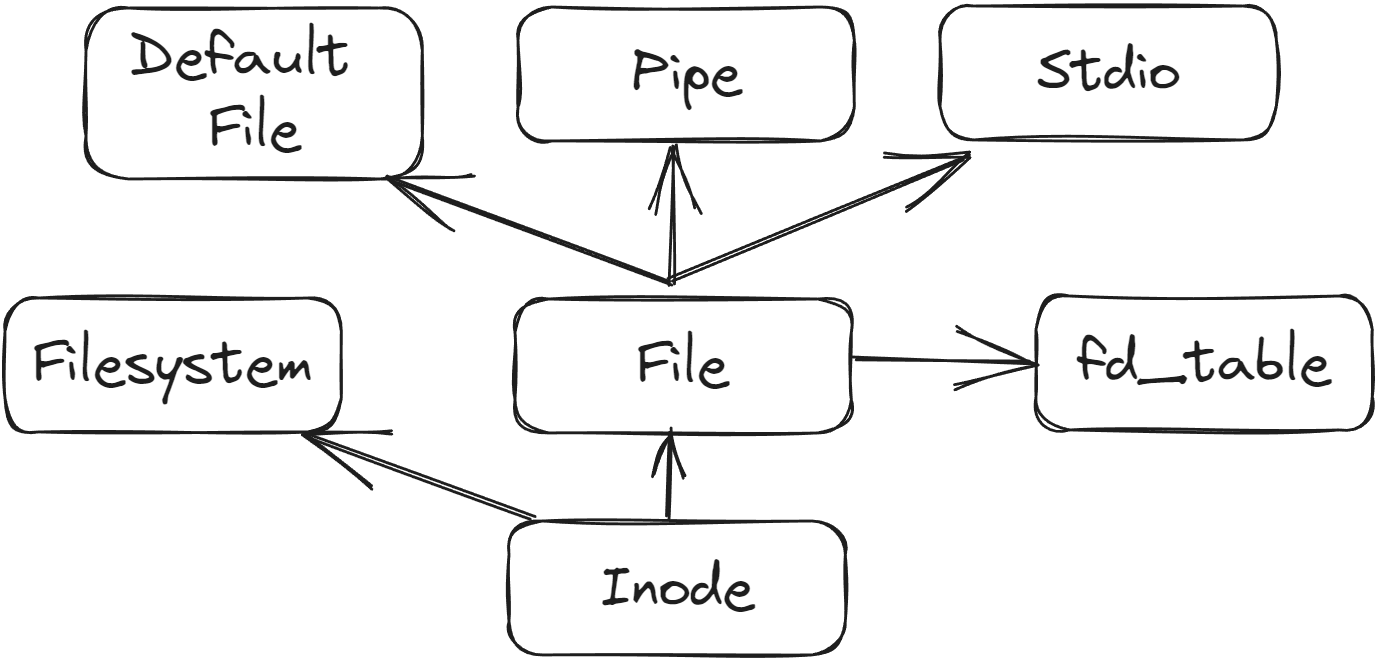
\includegraphics[width=.8\linewidth]{figure/vfs_layout.png}
    \caption{VFS框架}
    \label{pic:vfs_layout}
\end{figure}

对于Inode,由于Titanix中不存在dentry的概念,原本由dentry的负责的路径转实际inode的过程(lookup),现在应该交由inode负责。于是为了后续对inode内容的更改的便捷,我们设计了以下InodeMeta结构体:

% \newenvironment{codebox}[1]{
% \begin{tcolorbox}[title=\textbf{#1}]
% \begin{minted}{rust}
% }{
% \end{tcolorbox}
% }

% \begin{codebox}{xxxxstruct}
% pub struct jiwjjowjiwojofiew {
%     pub fuck: usize,
% }
% \end{minted}
% \end{codebox}


\begin{tcolorbox}[
title=\textbf{os/src/fs/inode.rs},
listing only,
breakable
]
\begin{minted}[breaklines, baselinestretch=1, fontsize=\small]{rust}
pub struct InodeMeta {
    /// inode number
    pub ino: usize,
    /// data address
    pub data: usize,
    /// type of inode
    pub mode: InodeMode,
    /// device id (only for block device and char device)
    pub rdev: Option<usize>,
    /// inode's device
    pub device: Option<InodeDevice>,
    /// path to this inode
    pub path: String,
    /// name which doesn't have slash
    pub name: String,
    /// a inode's unique id
    pub uid: usize,
    pub inner: Mutex<InodeMetaInner>,
}
\end{minted}
\end{tcolorbox}

并将可能需要更改的对象放在了IndoeMetaInner里面,这里给出InodeMetaInner结构体的设计:

\begin{tcolorbox}[
title=\textbf{os/src/fs/inode.rs},
listing only,
breakable
]
\begin{minted}[breaklines, baselinestretch=1, fontsize=\small]{rust}
pub struct InodeMetaInner {
    // pub offset: usize,
    /// inode' file's size
    pub size: usize,
    /// last access time, need to flush to disk.
    pub st_atim: TimeSpec,
    /// last modification time, need to flush to disk
    pub st_mtim: TimeSpec,
    /// last status change time, need to flush to disk
    pub st_ctim: TimeSpec,
    /// hash name(Note that this doesn't consider the parent uid)
    pub hash_name: HashName,
    /// parent
    pub parent: Option<Weak<dyn Inode>>,
    /// brother list
    pub brothers: BTreeMap<String, Weak<dyn Inode>>,
    /// children list
    pub children: BTreeMap<String, Arc<dyn Inode>>,
    /// page cache of the related file
    pub page_cache: Option<PageCache>,
    /// data len
    pub data_len: usize,
}
\end{minted}
\end{tcolorbox}

为什么要这样做呢?这是考虑到rust这门语言的特性。rust对于对象的可变性有着较高的要求,对于可变对象的可变引用,如果想要保证对象在并行线程之间的访问的安全性,需要使用智能指针来保证(我们使用Arc来将可能需要更改的对象包裹),但是智能指针(Arc)要求对象为不可变,这样的话,如果想要更改对象的值,我们只能通过unsafe块来包裹线程不安全的代码,并自己手动保证线程之间的访问安全。我们最开始是这样写的,但是后面发现这样会导致代码难以读懂,并且导致指针之间的关系复杂且曲折。实际上,这种写法是违背rust的特性的。rust这门语言希望你不要随意对Arc中的对象进行更改,如果一定需要,请``上锁"。那么有什么办法可以对某一对象在保持Arc的引用的同时还可以更改其中的某些一值?答案就是将这些可能需要更改的对象抽象出来,作为一个Inner对象,并在原来的对象中添加该Inner对象,但是需要用所来包裹保证更改时的线程安全,这样就有了我们的解决办法。

这样做还有另外一个好处,通过将可变对象和不可变对象分开,使得我们可以在访问可变对象的同时,只对Inner上锁,让外部的不可变对象的访问可以并行执行,极大的提高了访问的并行性。

\paragraph{Name Hash}~{}

由于文件系统的文件组织具有层次化的特点,往往都会存在父目录和子目录这样的关系,所以在Linux当中,对于文件查找,使用了哈希表的技术来加快文件名到对应的inode的查找。

Titanix效仿Linux,同样对inode和实际文件名(字符串类型)之间建立一层哈希映射,以便于快速地进行文件查找。为此我们设计了HashName结构体,该结构体完成了文件名(str类型)到u64类型的映射,当我们知道文件名之后,就可以调用该结构体实现的hash\_name方法进行哈希值的计算,并从构建的全局哈希表当中获取该inode的Arc引用。该结构体如下所示:

\begin{tcolorbox}[
title=\textbf{os/src/fs/hash\_name.rs},
listing only,
breakable
]
\begin{minted}[breaklines, baselinestretch=1, fontsize=\small]{rust}
#[derive(Clone, PartialEq)]
pub struct HashName {
    pub name_hash: u64,
    pub parent: usize,
    pub name: Arc<str>,
}
\end{minted}
\end{tcolorbox}

你可能注意到了,我们的HashName结构体中存在parent的字段,为什么要设置这个字段呢?这是因为文件系统的层次性让我们可以在文件查询的时候做一些``小手脚"。通常来将,我们查找文件是将以字符串标识的路径,转换成对应的inode,那么这个过程可以通过从根inode开始进行逐层查找,所以一般来讲,我们是通过父目录找到下一级的目录,然后逐级查找到对应的文件(inode),那么我们就可以使用父目录和子目录的名字来一起做哈希,这样可以使得我们的哈希能够铺得更加平,从而在查找的时候能够在更加小的范围内进行精确匹配,使得查找的速度加快。

为了实现该结构体的一些hash函数,我们参考了Github开源仓库rust-hash-table中对于哈希表的实现。核心方法hash\_name的实现如下:
\begin{tcolorbox}[
title=\textbf{os/src/fs/hash\_name.rs},
listing only,
breakable
]
\begin{minted}[breaklines, baselinestretch=1, fontsize=\small]{rust}
pub fn hash_name(parent: Option<usize>, name: &str) -> HashName {
    let parent_ptr = match parent {
        Some(p) => p as u64,
        None => 0 as u64,
    };
    HashName {
        name_hash: Self::myhash(parent_ptr, Self::str2num(name)),
        parent: parent_ptr as usize,
        name: Arc::from(name),
    }
}
\end{minted}
\end{tcolorbox}

\paragraph{Inode Cache}~{}

通过Name Hash来加速查找可以提高查找的速度,但是频繁的访问磁盘永远不是一个好的决定,于是Titanix采用了一贯的用于协调内外存访问速度不匹配问题的解决办法——开辟缓存!

我们通过设置全局对象INODE\_CACHE,来对可能会使用的inode进行缓存,由于需要保证线程之间的并行访问安全,我们需要对该对象上锁。对于INODE\_CACHE,他应该完成某一个文件的inode的文件名哈希值与inode自身的映射管理,于是我们在设计Titanix时,将INODE\_CACHE定义为以下形式:
\begin{tcolorbox}[
title=\textbf{os/src/fs/inode.rs},
listing only,
breakable
]
\begin{minted}[breaklines, baselinestretch=1, fontsize=\small]{rust}
lazy_static! {
    pub static ref INODE_CACHE: Mutex<HashTable<usize, Arc<dyn Inode>>> = Mutex::new(HashTable::new());
}
\end{minted}
\end{tcolorbox}
可以看见,我们在申明该全局对象时,采用了lazy allocation的方式以帮助我们更好得实现内存管理,这里使用了rust的lazy\_static模块。

\paragraph{路径解析}~{}

对于路径解析,Titanix效仿Linux实现inode的lookup查找,利用文件名哈希值来加速查找,并利用INODE\_CACHE来减少访问磁盘的次数,我们给出了以下lookup方法:
\begin{tcolorbox}[
title=\textbf{os/src/fs/inode.rs},
listing only,
breakable
]
\begin{minted}[breaklines, baselinestretch=1, fontsize=\small]{rust}
fn lookup(&self, this: Arc<dyn Inode>, name: &str) -> Option<Arc<dyn Inode>> {
    let key = HashName::hash_name(Some(self.metadata().uid), name).name_hash as usize;
    let value = INODE_CACHE.lock().get(&key).cloned();
    match value {
        Some(value) => Some(value.clone()),
        None => {
            debug!(
                "cannot find child dentry, name: {}, try to find in inode",
                name
            );
            let target_inode = self.try_find_and_insert_inode(this, name);
            match target_inode {
                Some(target_inode) => Some(target_inode.clone()),
                None => None,
            }
        }
    }
}
\end{minted}
\end{tcolorbox}
从该方法的参数可以看出,这是一个成员函数,如何调用该方法呢?需要一个inode对象通过``."的方式来访问该成员方法。从这里就可以看出我们的lookup的逻辑,实际上是父亲inode调用lookup函数查找对应的孩子inode的过程。从上面的代码不难看出,我们会先尝试在INDOE\_CAHCE当中查找是否存在对应的inode,然后如果不存在,才开始调用try\_find\_and\_insert\_inode函数,试图在实际文件系统当中查找该inode,但是如果查找失败,那么返回值为None,交由上层判断处理。

对于try\_find\_and\_insert\_inode函数,我们将其作为VFS与实际文件系统相衔接的部分,这一方法负责调用VFS提供给实际文件系统的一些接口来实现从实际文件系统中查找对应的inode,由于调用该方法往往意味着在内存的INODE\_CACHE当中没有找到该inode,所以该方法顺带将找到的inode添加到INODE\_CACHE当中。以下给出该方法的代码:
\begin{tcolorbox}[
title=\textbf{os/src/fs/inode.rs},
listing only,
breakable
]
\begin{minted}[breaklines, baselinestretch=1, fontsize=\small]{rust}
fn try_find_and_insert_inode(
        &self,
        this: Arc<dyn Inode>,
        child_name: &str,
    ) -> Option<Arc<dyn Inode>> {
    let key = HashName::hash_name(Some(self.metadata().uid), child_name).name_hash as usize;
    self.load_children(this);
    debug!(
        "children size {}",
        self.metadata().inner.lock().children.len()
    );
    let target_inode = self
        .metadata()
        .inner
        .lock()
        .children
        .get(child_name)
        .cloned();
    match target_inode {
        Some(target_inode) => {
            // find the inode which related to this subdentry
            INODE_CACHE.lock().insert(key, target_inode.clone());
            Some(target_inode.clone())
        }
        None => {
            debug!("Cannot find {} in children", child_name);
            None
        }
    }
}
\end{minted}
\end{tcolorbox}
这里面的load\_children方法就是提供给实际文件系统的接口,用于向内存当中载入给定inode的孩子inode。

在上面单层查找的基础之上,我们实现了从根inode开始查找的代码:
\begin{tcolorbox}[
title=\textbf{os/src/fs/inode.rs},
listing only,
breakable
]
\begin{minted}[breaklines, baselinestretch=1, fontsize=\small]{rust}
/// Look up from root(e.g. "/home/oscomp/workspace")
    pub fn lookup_from_root(
        // file_system: Arc<dyn FileSystem>,
        path: &str,
    ) -> Option<Arc<dyn Inode>> {
    let path_names = Path::path2vec(path);
    let root_fs = FILE_SYSTEM_MANAGER
        .fs_mgr
        .lock()
        .get("/")
        .cloned()
        .expect("No root fs is mounted");
    let mut parent = root_fs.metadata().root_inode.clone().unwrap();
    for name in path_names {
        match parent.lookup(parent.clone(), name) {
            Some(p) => parent = p,
            None => return None,
        }
    }
    Some(parent)
}
\end{minted}
\end{tcolorbox}
该方法并不是一个关联方法,而是一个静态方法。抽象出该方法的目的是为了编写内核系统调用时能够更加有逻辑,并将大量重复代码进行复用。

\paragraph{文件系统抽象}~{}

Titanix为所有的文件系统建立一层抽象,通过让实际文件系统实现该FileSystem trait来将自己接入Titanix。为了在mount的时候能够区分不同的文件系统类型,Titanix将自己支持的文件系统类型直接硬编码到了内核当中,我们设计了FileSystemType这个枚举类型:
\begin{tcolorbox}[
title=\textbf{os/src/fs/file\_system.rs},
listing only,
breakable
]
\begin{minted}[breaklines, baselinestretch=1, fontsize=\small]{rust}
#[derive(Clone)]
pub enum FileSystemType {
    VFAT,
    EXT2,
    NFS,
}
impl FileSystemType {
    pub fn fs_type(ftype: String) -> Option<Self> {
        match ftype {
            vfat => Some(Self::VFAT),
            ext2 => Some(Self::EXT2),
            nfs => Some(Self::NFS),
            _ => None,
        }
    }
    pub fn new_fs(&self) -> impl FileSystem {
        match self {
            Self::VFAT => {
                // let fs = FAT32FileSystem::new();
                let fs = TestFs::new();
                fs
            }
            _ => {
                todo!()
            }
        }
    }
}
\end{minted}
\end{tcolorbox}
目前Titanix只能支持FAT32文件系统,后续还会支持更多类型的文件系统。

所有的文件系统通过实现Titanix中的FileSystem中的方法,可以实现与内核的对接,我们为实际文件系统实现了默认的初始化方法,但是这个只针对FAT32文件系统,后续还需要进行修改。实际文件系统通过将write\_inode、sync\_fs等方法实现来完成Titanix需要的文件交互动作。

\subsubsection{FAT32文件系统}